\documentclass{report}

\input{~/dev/latex/template/preamble.tex}
\input{~/dev/latex/template/macros.tex}

\title{\Huge{}}
\author{\huge{Nathan Warner}}
\date{\huge{}}
\pagestyle{fancy}
\fancyhf{}
\lhead{Warner \thepage}
\rhead{}
% \lhead{\leftmark}
\cfoot{\thepage}
\setborder
% \usepackage[default]{sourcecodepro}
% \usepackage[T1]{fontenc}

\begin{document}
    % \maketitle
        \begin{titlepage}
       \begin{center}
           \vspace*{1cm}
    
           \textbf{Chapters 9-12} \\
    
           \vspace{0.5cm}
           Stat 128: Elementary Statistics
            
                
           \vspace{1.5cm}
    
           \textbf{Nathan Warner}
    
           \vfill
                
                
           \vspace{0.8cm}
         
           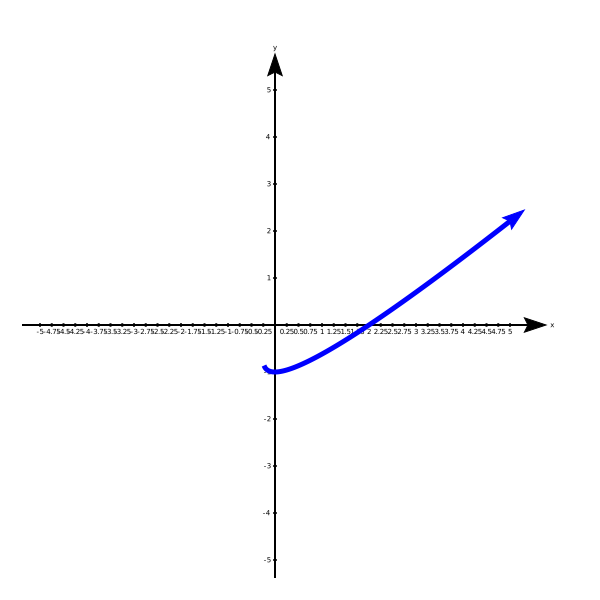
\includegraphics[width=0.4\textwidth]{/home/datura/dormprep/figures/1.png}
                
           Computer Science \\
           Northern Illinois University\\
           United States\\
           July 27, 2023
           
                
       \end{center}
    \end{titlepage}
    \tableofcontents
    \pagebreak \bigbreak \noindent
    \begin{center}
        \phantomsection
        \addcontentsline{toc}{section}{Chapter 9}
        \section*{Chapter 9}
    \end{center}
    \line(1,0){490}
    \bigbreak \noindent 
    \subsection{9.1 Estimating a Population Proportion}
    \bigbreak \noindent \bigbreak \noindent  
    \textbf{\textit{\underline{Learning Objectives For This Section:}}}
    \begin{enumerate}
        \item \textbf{Obtain a Point Estimate for the Population Proportion}
        \item \textbf{Construct and Interpret a Confidence Interval for the Population Proportion}
        \item \textbf{Determine the Sample Size Necessary for Estimating a Population Proportion within a Specified Margin of Error}
    \end{enumerate}
    \bigbreak \noindent \bigbreak \noindent 
    \textbf{Vocab:}
    \begin{itemize}
        \item A \textbf{point estimate} is the value of a statistic that estimates the value of a parameter.
        \item \textbf{A Confidence Interval} for an  unknown parameter consists of an interval of numbers based on a point estimate.
        \item \textbf{The level of confidence} represents the expected proportion of intervals that will contain the parameter if a large number of different samples is obtained.
        \item \textbf{Critical Value} represents the number of standard deviations the sample statistic can be from the parameter and still result in an interval that includes the parameter.
    \end{itemize}
    \bigbreak \noindent \bigbreak \noindent 
    \textbf{Formulas/Notation:}
    \begin{itemize}
        \item \textbf{Point Estimate = Sample Proportion}
            \begin{align*}
                \hat{p} = \frac{x}{n}
            .\end{align*}
        \item The \textbf{Margin of Error} is denoted:
            \begin{align*}
                E 
            .\end{align*}
        \item \textbf{Confidence Intervals for a Proportion} are of the form:
            \begin{center}
                point estimate $\pm $ margin of error
            \end{center}
            That is:
            \begin{align*}
               \hat{p} \pm E 
            .\end{align*}
            We have 95\% confidence that the sampling proportion will lie between:
            \begin{align*}
                \hat{p} \pm 1.96 \sigma_{\hat{p}}  
            .\end{align*}
        \item \textbf{The level of confidence} is denoted:
            \begin{align*}
                (1-\alpha) \cdot 100\%
            .\end{align*}
        \item \textbf{Standard Error:}
            \begin{align*}
                \sigma_{\hat{p}} = \sqrt{\frac{\hat{p}(1-\hat{p})}{n}}
            .\end{align*}
        \item \textbf{Constructing any (1−$\alpha $)$\cdot  $100\% Confidence Interval}
            \begin{align*}
                \hat{p} - z_{\alpha/2} \cdot \sqrt{\frac{\hat{p}(1-\hat{p})}{n}} < p < \hat{p} + z_{\alpha/2} \cdot \sqrt{\frac{\hat{p}(1-\hat{p})}{n}}
            .\end{align*}

        \item \textbf{Critical Value}
            \begin{align*}
                z_{ \frac{\alpha}{2}}
            .\end{align*}
            \bigbreak \noindent \bigbreak \noindent
        \end{itemize}

        \pagebreak \bigbreak \noindent 
        \begin{itemize}
            \item  \textbf{Constructing a (1−$\alpha $)$\cdot$ 100\% Confidence Interval for a Population Proportion:}
            Suppose that a simple random sample of size $n $ is taken from a population or the data are the result of a randomized experiment. A (1−$\alpha $)$\cdot  $100\% confidence interval for $p $ is given by the following quantities:
          \begin{align*}
              Lower\ bound:\ \hat{p} - z_{\frac{\alpha}{2}} \cdot \sqrt{\frac{\hat{p}(1 - \hat{p})}{n}}  \\
              Upper\ bound:\ \hat{p} + z_{\frac{\alpha}{2}} \cdot \sqrt{\frac{\hat{p}(1 - \hat{p})}{n}}
          .\end{align*}
          \textbf{Note:} It must be the case that $n\hat{p}(1-\hat{p})\geq 10$ and $n \leq 0.05N$ to construct this interval. Use $\hat{p}$ in place of $p$ in the standard deviation. This is because $p$ is unknown, and $\hat{p}$ is the best point estimate of $p$.
          \item The \textbf{margin of error}, $E $, in a (1−$\alpha $)$\cdot  $100\% confidence interval for a population proportion is given by
          \begin{align*}
              E = Z_{\frac{\alpha}{2}} \cdot \sqrt{\frac{\hat{p}(1-\hat{p})}{n}} \\
              or:\ \frac{Upper\ Limit\ - Lower\ Limit}{2}
          .\end{align*}
      \item \textbf{Sample Size Needed for Estimating the Population Proportion}
          \begin{align*}
              n = \hat{p} \cdot (1 - \hat{p}) \cdot \left(\frac{z_{\alpha/2}}{E}\right)^2 
          .\end{align*}
          (rounded up to the next integer) where $\hat{p}$ is a prior estimate of p.
          \bigbreak \noindent 
          If a prior estimate of p is unavailable, the sample size required is
          \begin{align*}
              n = 0.25 \cdot \left(\frac{z_{\alpha/2}}{E}\right)^2
          .\end{align*}
          rounded up to the next integer. The margin of error should always be expressed as a decimal when using these formulas.
        \item \textbf{Width}
            \begin{align*}
                2(E)
            .\end{align*}
      \end{itemize}


    \pagebreak \bigbreak \noindent 
    \textbf{\textit{\underline{Introduction}}}
    \bigbreak \noindent 
    \textbf{Two Types of Inferential Statistics:}
    \begin{enumerate}
        \item Estimation
        \item Hypothesis Testing
    \end{enumerate}

    \bigbreak \noindent \bigbreak \noindent 
    \textbf{\textit{\underline{Obtain a Point Estimate for the Population Proportion}}}
    \bigbreak \noindent 
    Suppose we want to estimate the proportion of adult Americans who believe that the amount they pay in federal income taxes is fair. It is unreasonable to expect that we could survey every adult American. Instead, we use a sample of adult Americans to arrive at an estimate of the proportion. We call this estimate a point estimate.
    \bigbreak \noindent 
    \begin{mdframed}
      \textbf{Example: }
      \bigbreak \noindent 
      \textbf{Problem:}
      \bigbreak \noindent 
      The Gallup Organization conducted a poll in April 2017 in which a simple random sample of 1019 Americans aged 18 and older were asked, “Do you regard the income tax that you will have to pay this year as fair?” Of the 1019 adult Americans surveyed, 620 said yes. Obtain a point estimate for the proportion of Americans aged 18 and older who believe that the amount of income tax they pay is fair.
      \bigbreak \noindent 
      \textbf{Approach:}
      The point estimate of the population proportion is $\hat{p}=\frac{x}{n}$, where $x=620$ and $n=1019$.
      \bigbreak \noindent 
      \textbf{Solution:}
      \bigbreak \noindent 
      Substituting into the formula, we get $\hat{p}=\frac{x}{n}=\frac{620}{1019}=0.608=60.8\%$.
      \bigbreak \noindent 
        We estimate that 60.8\% of Americans aged 18 and older believe that the amount of income tax they pay is fair.
    \end{mdframed}

    \bigbreak \noindent \bigbreak \noindent 
    \textbf{\textit{\underline{Construct and Interpret a Confidence Interval for the Population Proportion}}}
    \bigbreak \noindent 
    What if we conducted a different random sample of 1019 Americans aged 18 years or older? Would we get the same sample proportion who believe the amount of income tax they pay is fair? Probably not. Why? Because statistics such as $\hat{p}$ vary from sample to sample. So a different random sample of adult Americans might result in a different point estimate of the population proportion, such as $\hat{p}=0.593$.
    \bigbreak \noindent 
    If the method used to select the adult Americans was done appropriately, both point estimates would be good guesses of the population proportion. Due to variability in the sample proportion, we report a range (or interval) of values, including a measure of the likelihood that the interval includes the unknown population proportion.
    \bigbreak \noindent
    Consider the following:
    \begin{align*}
        \hat{p} = 0.54 \quad E = 0.034
    .\end{align*}
    Then:
    \begin{align*}
        0.54 - 0.034 = 0.506 \\
        0.54 + 0.034 = 0.574
    .\end{align*}
    With this we can say "We are 95\% confident that the proportion is between 0.506 and 0.574"
    \pagebreak \bigbreak \noindent 
    Figure:
    \bigbreak \noindent \bigbreak \noindent 
    \begin{figure}[ht]
        \centering
        \incfig{figmanea}
        \label{fig:figmanea}
    \end{figure}
    \bigbreak \noindent 
    Where does the 1.96 comes from?
    \begin{align*}
        z_{\alpha} \\
        z_{0.025} = 1.96
    .\end{align*}
    \bigbreak \noindent \bigbreak \noindent 
    This graphic also infers that 95\% of all sample proportions will lie between:
    \begin{align*}
        p-1.96\sigma_{\hat{p}} < \hat{p} < p +1.96\sigma_{\hat{p}}
    .\end{align*}
    \bigbreak \noindent \bigbreak \noindent 
    By solving this inequality such that $p $ is in the center:
    \begin{align*}
        \hat{p} -1.96\sigma_{\hat{p}} < p < \hat{p}  + 1.96 \sigma_{\hat{p}}
    .\end{align*}
    \bigbreak \noindent 
    And we can write this in shorthand form:
    \begin{align*}
        \hat{p} \pm 1.96 \sigma_{\hat{p}} \\
        or:\ \hat{p} \pm E
    .\end{align*}
    \bigbreak \noindent 
    \textit{figure:}
    \bigbreak \noindent 
\begin{figure}[ht]
    \centering
    \incfig{fuga}
    \label{fig:fuga}
\end{figure}

    \pagebreak \bigbreak \noindent 
    \textbf{Summary:}
    \bigbreak \noindent 
    \begin{itemize}
        \item for a 95\% confidence interval, any sample proportion that lies withing 1.96 standard errors of the population proportion will result in a confidence interval that includes $p $. This will happen in 95\% of all possible samples.
        \item Any sample proportion that is more than 1.96 standard errors from the population proportion will result in a confidence interval that does not contain $p $. This will happen in 5\% of all possible samples (those sample proportions in the tails of the distribution).
        \item A confidence interval for an unknown parameter consists of an interval of numbers based on a point estimate.
        \item The level of confidence represents the expected proportion of intervals that will contain the parameter if a large number of different samples is obtained. The level of confidence is denoted (1−$\alpha $)$\cdot $ 100\%.
        \item Whether a confidence interval contains the population parameter depends solely on the value of the sample statistic. Any sample statistic that is in the tails of the sampling distribution will result in a confidence interval that does not include the population parameter. See Figure 1. Notice that $\hat{p}_1$ results in a confidence interval that includes the population proportion, $p$. However, $\hat{p}_2$ results in a confidence interval that does not include the population proportion, $p$, because $\hat{p}_2$ is in the tails of the distribution.
    \end{itemize}

    \bigbreak \noindent \bigbreak \noindent 
    \qs{}{The horizontal axis in the sampling distribution of  represents all possible sample proportions from a simple random sample of size n. 
        \bigbreak \noindent 
        \textbf{a.) What percent of sample proportions results in a ​75\% confidence interval that includes the population​ proportion?}
        \smallbreak \noindent
        \textbf{b.) What percent of sample proportions results in a ​75\% confidence interval that does not include the population​ proportion?}
        \bigbreak \noindent 
        \pf{Solution:}{}
        \textbf{a.)} 75\%
        \smallbreak \noindent
        \textbf{b.)} 25\%
}
    \bigbreak \noindent 
    \textbf{Caution:}
    \bigbreak \noindent 
    95\% confident does not mean 95\% probability. Probability describes the likelihood of undetermined event.
    \bigbreak \noindent 
    It does not make sense to talk about the probability that the interval contains the parameter, because the parameter is an unknown, but fixed value. Thus, it is either in the interval, or not. 
    \bigbreak \noindent 
    Consider a coin flip, if a coin has been flipped but its outcome has not been revealed, the flip resulting in a head is not $\frac{1}{2} $, because the outcome has already been determined. Instead the probability is either $0$, or $1$
    \bigbreak \noindent 
    Therefore, the probability that any confidence interval contains a parameter is either $0$, or $1$.
    \bigbreak \noindent 
    We do say "we are 95\% confident the interval contains the parameter" because the method "works" in 95\% of all samples.

    \pagebreak \bigbreak \noindent 
    \textbf{Constructing any $(1-\alpha)\cdot 100\% $ Confidence interval}
    \bigbreak \noindent 
    We need a method for constructing any $(1-\alpha) \cdot 100\%$ confidence interval. When $\alpha=0.05$, we are constructing a $95\%$ confidence interval.
    \bigbreak \noindent 
    We generalize
    \begin{figure}[ht]
        \centering
        \incfig{construct}
        \label{fig:construct}
    \end{figure}
    \bigbreak \noindent 
    by first noting that $(1-\alpha)\cdot 100\%$  of all sample proportions are in the interval as shown in Figure 2.
    \bigbreak \noindent 
    \textit{Figure 2}
    \bigbreak \noindent 
    \begin{figure}[ht]
        \centering
        \incfig{const}
        \label{fig:const}
    \end{figure}
    \bigbreak \noindent 
    Rewrite this inequality with p in the middle and obtain
    \begin{align*}
        \hat{p} - z_{\frac{\alpha}{2}} \cdot \sqrt{\frac{\hat{p}(1 - \hat{p})}{n}} < p < \hat{p} + z_{\frac{\alpha}{2}} \cdot \sqrt{\frac{\hat{p}(1 - \hat{p})}{{n}}}
    .\end{align*}
    \bigbreak \noindent 
    So (1−$\alpha $)⋅100\% of all sample proportions will result in confidence intervals that contain the population proportion. The sample proportions that are in the tails of the distribution in Figure 2 will not result in confidence intervals that contain the population proportion.

    \pagebreak \bigbreak \noindent 
    Table 1 shows some of the common critical values used in the construction of confidence intervals. Notice that higher levels of confidence correspond to higher critical values. After all, if your level of confidence that the interval includes the unknown parameter increases, the width of your interval (through the margin of error) should increase.
    \begin{center}
        \begin{center}
            \begin{tabular}{|l|c|c|}
            \hline
            Level of confidence $(1-\alpha) \cdot 100\%$ & Area in each tail $\frac{\alpha}{2}$ & Critical Value $z_{\frac{\alpha}{2}}$ \\
            	\hline
            90\% & 0.05 & 1.645   \\
            	\hline
            95\% & 0.025 & 1.96 \\
            \hline 
            99\% & 0.005 & 2.575 \\
            \hline
            \end{tabular}
        \end{center}
    \end{center}

    \bigbreak \noindent 
    \textbf{Interpretation of a Confidence Interval }
    \bigbreak \noindent 
    A $(1-\alpha)\cdot 100\%$ confidence interval indicates that $(1-\alpha)\cdot 100\%$ of all simple random samples of size $n$ from the population whose parameter is unknown will result in an interval that contains the parameter.
    \bigbreak \noindent 
    For example, a 90\% confidence interval for a parameter suggests that 90\% of all possible samples will result in an interval that includes the unknown parameter and 10\% of the samples will result in an interval that does not capture the parameter.
    \begin{mdframed}
      \textbf{Example: Interpreting a Confidence Interval}
      \bigbreak \noindent 
      \textbf{Problem:}
      The Gallup Organization conducted a poll in April 2017 in which a simple random sample of 1019 Americans aged 18 and older were asked, “Do you regard the income tax that you will have to pay this year as fair?” We learned from Example 1 that the proportion of those surveyed who responded yes was 0.608. Gallup reported its “survey methodology” as follows:
      \bigbreak \noindent 
      \textbf{Approach:}
      Confidence intervals for a proportion are of the form point estimate ± margin of error. So add and subtract the margin of error from the point estimate to obtain the confidence interval. Interpret the confidence interval, ”We are 95\% confident that the proportion of Americans aged 18 and older who believe that the income tax they will have to pay this year is fair is between lower bound and upper bound.”
      \bigbreak \noindent 
      \textbf{Solution:}
      \bigbreak \noindent 
      The point estimate is 0.608, and the margin of error is 0.04. The confidence interval is $0.608 \pm 0.04$. Therefore, the lower bound of the confidence interval is $0.608 - 0.04 = 0.568$ and the upper bound of the confidence interval is $0.608 + 0.04 = 0.648$. We are 95\% confident that the proportion of Americans aged 18 and older who believe that the income tax they will have to pay this year is between 0.568 and 0.648.
      \bigbreak \noindent 
    \end{mdframed}
    \bigbreak \noindent 
      \textbf{We are now prepared to present a method for constructing a confidence interval about the population proportion, $p $}
      \bigbreak \noindent 
      \textbf{Constructing a (1−$\alpha $)⋅100\% Confidence Interval for a Population Proportion:}
      \bigbreak \noindent 
      Suppose that a simple random sample of size $n $ is taken from a population or the data are the result of a randomized experiment. A (1−$\alpha $)⋅100\% confidence interval for $p $ is given by the following quantities:
      \begin{align*}
          Lower\ bound:\ \hat{p} - z_{\frac{\alpha}{2}} \cdot \sqrt{\frac{\hat{p}(1 - \hat{p})}{n}}  \\
          Upper\ bound:\ \hat{p} + z_{\frac{\alpha}{2}} \cdot \sqrt{\frac{\hat{p}(1 - \hat{p})}{n}}
      .\end{align*}
      \bigbreak \noindent 
      \nt{It must be the case that $n\hat{p}(1-\hat{p})\geq 10$ and $n \leq 0.05N$ to construct this interval. Use $\hat{p}$ in place of $p$ in the standard deviation. This is because $p$ is unknown, and $\hat{p}$ is the best point estimate of $p$.}

      \pagebreak \bigbreak \noindent 
      \bigbreak \noindent 
      \begin{mdframed}
        \textbf{Example: Constructing a Confidence Interval for a Population Proportion (Statcrunch)}
        \bigbreak \noindent 
        \textbf{Problem:}
        In the Parent–Teen Cell Phone Survey conducted by Princeton Survey Research Associates International, 800 randomly sampled 16- to 17-year-olds living in the United States were asked whether they have ever used their cell phone to text while driving. Of the 800 teenagers surveyed, 272 indicated that they text while driving. Obtain a 95\% confidence interval for the proportion of 16- to 17-year-olds who text while driving.
        \bigbreak \noindent 
        \textbf{Approach:}
        It is important to verify the requirements for constructing the confidence interval first. It must be the case that $n\hat{p}(1 −\hat{p}) \geq 10$ and the sample size is no more than 5\% of the population size (n $ \leq $0.05N).Then, construct the confidence interval either by hand or using technology.
        \bigbreak \noindent 
        \textbf{Solution:}
        \bigbreak \noindent 
        First, we obtain $\hat{p} $
        \begin{align*}
            \hat{p} = \frac{272}{800} = .34
        .\end{align*}
        \bigbreak \noindent 
        Verify Necessary Conditions:
        \begin{align*}
           n\hat{p}(1-\hat{p})  \geq 10 \\
            800(.34)(.66) = 179.52 \geq 10
        .\end{align*}
        \bigbreak \noindent 
        Also, we know that $n \leq0.05N $:
        \bigbreak \noindent 
        now in statcrunch:
        \begin{enumerate}
            \item Stat $>$ Proportion Stats $> $ One Sample $> $ with summary
            \item Input no. of successes
            \item Input no. of observations
            \item Input confidence level
            \item Method: Standard-Wald
            \item Compute
        \end{enumerate}
        \bigbreak \noindent 
        after doing the StatCrunch steps, we get a result of 0.307 and 0.373, therefore, we can conclude that we are 95\% confident that the proportion of 16 to 17-year-olds who text while driving is between 0.307 and 0.373

      \end{mdframed}

      \pagebreak \bigbreak \noindent 
        \begin{mdframed}
        \textbf{Example: Constructing a Confidence Interval for a Population Proportion (By hand)}
        \bigbreak \noindent 
        \textbf{Problem:}
        In the Parent–Teen Cell Phone Survey conducted by Princeton Survey Research Associates International, 800 randomly sampled 16- to 17-year-olds living in the United States were asked whether they have ever used their cell phone to text while driving. Of the 800 teenagers surveyed, 272 indicated that they text while driving. Obtain a 95\% confidence interval for the proportion of 16- to 17-year-olds who text while driving.
        \bigbreak \noindent 
        \textbf{Approach:}
        It is important to verify the requirements for constructing the confidence interval first. It must be the case that $n\hat{p}(1 −\hat{p}) \geq 10$ and the sample size is no more than 5\% of the population size (n $ \leq $0.05N).Then, construct the confidence interval either by hand or using technology.
        \bigbreak \noindent 
        \textbf{Solution:}
        \bigbreak \noindent 
        First, we obtain $\hat{p} $
        \begin{align*}
            \hat{p} = \frac{272}{800} = .34
        .\end{align*}
        \bigbreak \noindent 
        Verify Necessary Conditions:
        \begin{align*}
           n\hat{p}(1-\hat{p})  \geq 10 \\
            800(.34)(.66) = 179.52 \geq 10
        .\end{align*}
        \bigbreak \noindent 
        Also, we know that $n \leq0.05N $:
        \bigbreak \noindent 
        Now, to use the formula:
        \begin{align*}
            \hat{p} \pm E \\
        Where\ E = z_{\frac{\alpha}{2}} \cdot \sqrt{\frac{\hat{p}(1-\hat{p})}{n}}
        .\end{align*}
        We will need to find alpha, given that the formula for confidence level is:
        \begin{align*}
            (a-\alpha) \cdot 100\% \\
            1- \alpha = 0.95 \\
            \alpha = 0.05
        .\end{align*}
        \bigbreak \noindent 
        So our critical value is:
        \begin{align*}
            z_{\frac{\alpha}{2}} = z_{\frac{0.05}{2}} \\
            = z_{0.025}
        .\end{align*}
        Using the normal distribution table, we get:
        \begin{align*}
            \alpha = 1.96
        .\end{align*}
        \bigbreak \noindent 
        Now we can compute our bounds:
        \begin{align*}
            LB:\ = \hat{p} - z_{\frac{\alpha}{2}} \cdot \sqrt{\frac{\hat{p}(1-\hat{p})}{n}} \\
            = 0.34 - 19.6 \cdot \sqrt{\frac{0.34(0.66)}{800}} \\
            = 0.307 \\
            UB = \hat{p} + z_{\frac{\alpha}{2}} \cdot \sqrt{\frac{\hat{p}(1-\hat{p})}{n}} \\
            =0.34 + 1.96 \cdot \sqrt{\frac{0.34(0.66)}{800}} \\
            = 0.373
        .\end{align*}
        \bigbreak \noindent 
        Therefore:
        \begin{align*}
            Upper\ bound:\ 0.307 \quad Upper\ Bound:\ 0.373 \\
            Or: (0.307,0.373)
        .\end{align*}

    \end{mdframed}


    \bigbreak \noindent \bigbreak \noindent 
      \textbf{The Effect of Level of Confidence on the Margin of Error}
      \bigbreak \noindent 
      \begin{mdframed}
          \textbf{Example: The Role of the Level of Confidence in the Margin of Error} 
          \bigbreak \noindent 
          \textbf{Problem:}
          In the Parent--Teen Cell Phone Survey conducted by Princeton Survey Research Associates International, 800 randomly sampled 16- to 17-year-olds living in the United States were asked whether they have ever used their cell phone to text while driving. Of the 800 teenagers surveyed, 272 indicated that they text while driving. From the last example, we concluded that we are 95\% confident that the proportion of 16- to 17-year-olds who text while driving is between 0.307 and 0.373. Determine the effect on the margin of error by increasing the level of confidence from 95\% to 99\%.
          \bigbreak \noindent 
          \textbf{Approach:}
          We would expect the margin of error to increase with a larger level of confidence. Construct the confidence interval either by hand or using technology.
          \bigbreak \noindent 
          \textbf{Solution:}
          \bigbreak \noindent 
          The margin of error for the 95\% confidence interval found in Example 3 is 0.033, and the margin of error for the 99\% confidence interval is 0.043. So increasing the level of confidence increases the margin of error, resulting in a wider confidence interval.
      \end{mdframed}
      \bigbreak \noindent \bigbreak \noindent 
      \textbf{The Effect of Sample Size on the Margin of Error}
      \bigbreak \noindent 
      We know that larger sample sizes produce more precise estimates (the Law of Large Numbers). Given that the margin of error is $E=z_{\alpha/2} \cdot \hat{p} \cdot \sqrt{\frac{(1-\hat{p})}{n}}$, we can see that increasing the sample size $n$ decreases the standard error, so the margin of error decreases. Therefore, larger sample sizes will result in narrower confidence intervals.
      \bigbreak \noindent 
      \textbf{What If We Do Not Satisfy the Normality Condition?}
      \bigbreak \noindent 
     When the normality condition is not satisfied, the proportion of intervals that capture the parameter is below the level of confidence.

     \pagebreak \bigbreak \noindent 
     \textbf{\textit{Determine the Sample Size Necessary for Estimating a Population Proportion within a Specified Margin of Error}}
     \bigbreak \noindent 
     \begin{mdframed}
       \textbf{Example: Determining Sample Size}
       \bigbreak \noindent 
       \textbf{Problem:}
       An economist wants to know if the proportion of the U.S. population who commutes to work via car-pooling is on the rise. What size sample should be obtained if the economist wants an estimate within 2 percentage points of the true proportion with 90\% confidence?
       \bigbreak \noindent 
       Assume that the economist uses the estimate of 10\% obtained from the American Community Survey.
       \bigbreak \noindent 
       \textbf{Approach:}
       Since \(1 - \alpha = 0.9\), we know that \(\alpha = 0.10\). Use \(E = 0.02\), \(z_{\alpha/2} = z_{0.12} = z_{0.05} = 1.645\), and \(\hat{p} = 0.10\) (the prior estimate).
       \bigbreak \noindent 
       \textbf{Solution:}
       Using the formula assuming that a prior estimate is available, \(n = \hat{p}(1 - \hat{p})\left(\frac{z_{\alpha/2}}{E}\right)^2\), we obtain
       \begin{align*}
           n = \hat{p}(1 - \hat{p})\left(\frac{z_{\alpha/2}}{E}\right)^2 = 0.10 \times (1 - 0.10) \times \left(\frac{1.645}{0.02}\right)^2 = 608.9 
       .\end{align*}
       Round this value up to 609. So the economist must survey 609 randomly selected residents of the United States.
       \bigbreak \noindent 
       \textbf{statcrunch steps:}
       \bigbreak \noindent 
       First:
       \begin{align*}
           E = 0.02\ (\text{The 2 percentage points}) \\
           W = 2(E) = 0.04 \\
           C.Level = 0.9 \\
           Target\ Proportion = 0.1
       .\end{align*}
       \begin{enumerate}
           \item Stats $>$ Proportion Stats $>$ One Sample $> $ Width/Sample Size
            \item Input confidence level
            \item Input Target Proportion
            \item Compute
       \end{enumerate}
       \bigbreak \noindent 
       And we find that the minimum sample size would be 609
       \bigbreak \noindent 
       Now consider that the economist does not use any prior estimates (target proportion), in this case, our target proportion will be 0.5
       \bigbreak \noindent 
       With this target proportion we get 1691
     \end{mdframed}

     \pagebreak \bigbreak \noindent 
     \subsection{9.2: Estimating a Population Mean}
     \bigbreak \noindent 
     \textbf{\textit{\underline{Learning Objectives For This Section:}}}
     \begin{enumerate}
         \item \textbf{Obtain a Point Estimate for the Population Mean}
         \item \textbf{State Properties of Student’s t-Distribution}
         \item \textbf{Determine t-Values}
         \item \textbf{Construct and Interpret a Confidence Interval for a Population Mean}
         \item \textbf{Determine the Sample Size Necessary for Estimating a Population Mean within a Given Margin of Error}
     \end{enumerate}
     \bigbreak \noindent 
     \textbf{Vocab:}
     \begin{itemize}
         \item \textbf{The point estimate of the population mean}, $\mu$, is the sample mean, $\overline{x}$.
         \item \textbf{T-Interval:} confidence interval that uses the t-distribution
     \end{itemize}
     \bigbreak \noindent 
     \textbf{Notation/Formulas:}
     \begin{itemize}
        %  \item \textbf{Margin of error for population mean} 
        %      \begin{align*}
        %          z_{\frac{\alpha}{2}} \cdot \frac{\sigma}{\sqrt{n}}
        %      .\end{align*}
        % \item \textbf{Confidence Interval for population mean}
        %     \begin{align*}
        %         Point\ Estimate - Margin\ of\ Error \\
        %         = \overline{x} \pm z_{\frac{\alpha}{2}} \cdot \frac{\sigma}{\sqrt{n}} \\
        %         Or\ most\ likely = \overline{x} \pm z_{\frac{\alpha}{2}} \cdot \frac{s}{\sqrt{n}} \\
        %     .\end{align*}
        \item \textbf{Student’s t-distribution}
            \begin{align*}
               t = \frac{\overline{x}-\mu}{\frac{s}{\sqrt{n}}} 
            .\end{align*}
        \item \textbf{Constructing a (1−$\alpha $) $ \cdot $100\% Confidence Interval for $\mu$}
            Provided:
            \begin{itemize}
                \item sample data come from a simple random sample or randomized experiment
                \item sample size is small relative to the population size (n $ \leq $0.05N)
                \item the data come from a population that is normally distributed with no outliers, or the sample size is large
            \end{itemize}
            A (1−$\alpha $)$\cdot$100\% confidence interval for $\mu$ is given by
            \begin{align*}
                LB:\ = \overline{x}  - t_{\frac{\alpha}{2}} \cdot \frac{s}{\sqrt{n}} \\
                UB:\ = \overline{x}  + t_{\frac{\alpha}{2}} \cdot \frac{s}{\sqrt{n}} \\
            .\end{align*}
            where $t_{\frac{\alpha}{2}} $ is the critical value with n−1 degrees of freedom.
        \item \textbf{Margin of Error:}
            \begin{align*}
                E = t_{\frac{\alpha}{2}} \cdot \frac{s}{\sqrt{n}}
            .\end{align*}
        \item \textbf{Determine the Sample Size Necessary for Estimating a Population Mean within a Given Margin of Error}
            \begin{align*}
                n = \bigg(\frac{\frac{z_{\alpha}}{2}\cdot s}{E}\bigg)^{2}
            .\end{align*}
     \end{itemize}
     \pagebreak \bigbreak \noindent 
     \textbf{\textit{\underline{Obtain a Point Estimate for the Population Mean}}}
     \bigbreak \noindent 
     To find the point estimate of the population mean, compute the sample mean, $\overline{x} $

     \bigbreak \noindent \bigbreak \noindent 
     \textbf{\textit{\underline{State Properties of Student’s t-Distribution}}}
     \bigbreak \noindent 
     a different random sample of 16 cars would likely result in a different point estimate of $\mu$. For this reason, we want to construct a confidence interval for the population mean, just as we did for the population proportion.
     \bigbreak \noindent 
     A confidence interval for the population mean is of the form
     \begin{center}
         Point estimate $\pm $ Margin of Error
     \end{center}
     \bigbreak \noindent 
     (just like the confidence interval for a population proportion). To determine the margin of error, we need to know the sampling distribution of the sample mean.
     \bigbreak \noindent 
     Recall that the distribution of \(\bar{x}\) is approximately normal if the population from which the sample is drawn is normal or the sample size is sufficiently large. In addition, the distribution of \(\bar{x}\) has the same mean as the parent population, \(\mu_{\bar{x}} = \mu\), and a standard deviation equal to the parent population's standard deviation divided by the square root of the sample size, \(\sigma_{\bar{x}} = \frac{\sigma}{\sqrt{n}}\).
     \bigbreak \noindent 
     Following the same logic used in constructing a confidence interval about a population proportion, our confidence interval would be
     \begin{align*}
         point\ estimate \pm Margin\ of\ Error \\
         =  \bar{x} \pm z_{\frac{\alpha}{2}} \cdot \frac{\sigma}{\sqrt{n}}
     .\end{align*}
     \bigbreak \noindent 
     This presents a problem because we need to know the population standard deviation to construct this interval. It does not seem likely that we would know the population standard deviation but not know the population mean. So what can we do? A logical option is to use the sample standard deviation, \( s \), as an estimate of \( \sigma \). Then the standard deviation of the sampling distribution of \( \bar{x} \) would be estimated by \( \frac{s}{\sqrt{n}} \) and our confidence interval would be
     \begin{align*}
         \overline{x} \pm z_{\frac{\alpha}{2}} \cdot \frac{s}{\sqrt{n}}
     .\end{align*}
     \bigbreak \noindent 
     Unfortunately, there is a problem with this approach. The sample standard deviation, \( s \), is a statistic and therefore will vary from sample to sample. Using the normal model to determine the critical value, \( z_{\frac{\alpha}{2}} \), in the margin of error does not take into account the additional variability introduced by using \( s \) in place of \( \sigma \). This is not much of a problem for large samples because the variability in the sample standard deviation decreases as the sample size increases (Law of Large Numbers), but for small samples, we have a real problem.
     \bigbreak \noindent 
    Put another way, the z-score of \( \bar{x} \), \( \frac{\bar{x} - \mu}{\frac{\sigma}{\sqrt{n}}} \), is normally distributed with mean 0 and standard deviation 1 (provided \( \bar{x} \) is normally distributed). However, \( \frac{\bar{x} - \mu}{\frac{s}{\sqrt{n}}} \) is not normally distributed with mean 0 and standard deviation 1. So a new model must be used to determine the margin of error in a confidence interval that accounts for this additional variability. This leads to the story of William Gosset.
    \bigbreak \noindent 
    In the early 1900s, William Gosset worked for the Guinness brewery. Gosset was in charge of conducting experiments at the brewery to identify the best barley variety. When working with beer, Gosset was limited to small data sets. At the time, the model used for constructing confidence intervals about a mean was the normal model, regardless of whether the population standard deviation was known. Gosset did not know the population standard deviation, so he substituted the sample standard deviation for the population standard deviation and used the formula \(\bar{x} \pm z_{\frac{\alpha}{2}} \cdot \frac{s}{\sqrt{n}}\). While doing this, he was finding that his confidence intervals did not include the population mean at the rate expected. This led Gosset to develop a model that accounts for the additional variability introduced by using \( s \) in place of \( \sigma \) when determining the margin of error. Guinness would not allow Gosset to publish his results under his real name (Guinness was very secretive about its brewing practices), but did allow the results to be published under a pseudonym. Gosset chose "Student."

    \bigbreak \noindent 
    \begin{mdframed}
      \textbf{Definition: Student's T-Distribution}
      \bigbreak \noindent 
      We know that we can create a standard normal random variable, with the formula:
      \begin{align*}
          z = \frac{x - \mu}{s}
      .\end{align*}
      \bigbreak \noindent 
      Where $x $ is the value of the statistic, $\mu $ is the population mean, and $\sigma$ is the population standard deviation, Thus, if we wanted to created a standard normal random variable with a sample mean statistic, we would have the equation:
      \begin{align*}
          z = \frac{\overline{x} - \mu}{\frac{\sigma}{\sqrt{n}}}
      .\end{align*}
      \bigbreak \noindent 
      However this poses a problem, as states previously, we may not always know the value of $\sigma$, in this case, we can use students $t-distribution$, which states:
      \begin{align*}
           t = \frac{\overline{x} - \mu}{\frac{s}{\sqrt{n}}}
      .\end{align*}
      \bigbreak \noindent 
      So with the $t-distribution $, we are assuming we do not have access to $\sigma $.
      \bigbreak \noindent 
      It is important to note that when using students method, there will be additional variability in the $t-distribution$ compared to the $z-distribution $ 
    \end{mdframed}
    \bigbreak \noindent 
    \nt{Student's t-distribution is asymptotically normal, this means as the sample size n increases, student's t-distribution looks more and more like the standard normal distribution}

    \bigbreak \noindent 
    \textbf{Properties of the $t-distribution$}
    \begin{enumerate}
        \item The t-distribution is different for different degrees of freedom
        \item the t-distribution is centered at 0 and is symmetric about 0 
        \item The area under the curve is 1. The area around each curve to the right of 0 equals the area under the curve to the left of 0, which equals $1/2 $
     \item As t increases or decreases without bound, the graph approaches, but never equals, zero.
         \begin{align*}
             \lim\limits_{t \to -\infty}{f(x) = 0} \\
             \lim\limits_{t \to \infty}{f(x) = 0}
         .\end{align*}
        \item The area in the tails of the t-distribution is a little greater than the area in the tails of the standard normal distribution, because we are using $s $ as an estimate of $\sigma $, thereby introducing further variability into the t-statistic
        \item As the sample size $n $ increases, the density curve of $t $ get closer to the standard normal density curve. This result occurs because, as the sample size increases, the values of $s$ get closer to the value of $\sigma $, by the Law of Large Numbers.
    \end{enumerate}

    \pagebreak \bigbreak \noindent 
    \textbf{\textit{\underline{Construct and Interpret a Confidence Interval for a Population Mean}}}
    \bigbreak \noindent 
    We are now ready to construct a confidence interval for a population mean.
    \bigbreak \noindent 
    \textbf{Constructing a (1−$\alpha $)$\cdot $100\% Confidence Interval for $\mu$}
    \bigbreak \noindent 
    \textbf{Provided}
    \begin{itemize}
        \item sample data come from a simple random sample or randomized experiment
        \item sample size is small relative to the population size (n$\leq$0.05$N$)
        \item the data come from a population that is normally distributed with no outliers, or the sample size is large
    \end{itemize}
    \bigbreak \noindent 
    A (1−$\alpha$)$ \cdot  $100\% confidence interval for $\mu $ is given by:
    \begin{align*}
        Lower\ Bound:\ \overline{x} - t_{\frac{\alpha}{2}}\cdot \frac{s}{\sqrt{n}} \\
        Upper\ Bonud:\ \overline{x} + t_{\frac{\alpha}{2}}\cdot \frac{s}{\sqrt{n}} \\
    .\end{align*}
    \bigbreak \noindent 
    where $t_{\frac{\alpha}{2}} $ is the critical value with n−1 degrees of freedom.
    \bigbreak \noindent 
    Because this confidence interval uses the $t $-distribution, it is often referred to as the $t$-interval.
    \bigbreak \noindent 
    \nt{The margin of error is $E = t_{\frac{\alpha}{2}}\cdot \frac{s}{\sqrt{n}} $}
    \bigbreak \noindent 
    \textbf{A robust procedure}
    \bigbreak \noindent 
    Notice that a confidence interval about $\mu $ can be computed for non-normal populations even though Student’s t-distribution requires a normal population. This is because the procedure for constructing the confidence interval is robust—it is accurate despite minor departures from normality.
    \bigbreak \noindent 
    If a data set has outliers, the confidence interval is not accurate because neither the sample mean nor the sample standard deviation is resistant to outliers. Sample data should always be inspected for serious departures from normality and for outliers. This is easily done with normal probability plots and boxplots.
    \pagebreak \bigbreak \noindent 
    \begin{mdframed}
      \textbf{Example: Constructing a confidence interval about a population mean (By Hand)}
      \bigbreak \noindent 
      \textbf{Problem:}
    The website fueleconomy.gov allows drivers to report the miles per gallon of their vehicle. The data in Table 3 show the reported miles per gallon of 2011 Ford Focus automobiles for 16 different owners. Treat the sample as a simple random sample of all 2011 Ford Focus automobiles. Construct a 95\% confidence interval for the mean miles per gallon of a 2011 Ford Focus. Interpret the interval.
      \bigbreak \noindent 
      Before we begin, let's keep the following equation in mind:
      \begin{align*}
          \overline{x} \pm t_{\frac{\alpha}{2}}\cdot \frac{s}{\sqrt{n}}
      .\end{align*}
      \bigbreak \noindent 
      \textbf{Approach:} Before we begin, let's insure that the model requirements for constructing a confidence interval about a mean are satisfied by drawing a normal probability plot and boxplot.
      \bigbreak \noindent 
      We can confidently conclude that the data was obtained randomly, and the sample size 16 is much less than 5\% of the population size
      \bigbreak \noindent 
      Because the sample size is small, we first need to verify that the data came from a population that is \textit{normally distributed}, and also that the sample has not outliers. If we take a lot at the probability plot, we can see that the data is roughly linear, which insinuates that the data did indeed come from a population that is \textit{normally distributed}, furthermore, if we examine the boxplot, it becomes obvious that there are no outliers in the data.
      \bigbreak \noindent 
      Using technology, we can compute the sample mean $\overline{x} $ and the sample standard deviation $s $
      \begin{align*}
          \overline{x} = 36.8 \\
           s = 2.92
      .\end{align*}
      \bigbreak \noindent 
      Now let's find the critical value for the $t-distribution$
      \begin{align*}
          (1-\alpha) = 0.95 \\
          \alpha = 0.05 \\
          \frac{\alpha}{2} = 0.025 \\
      .\end{align*}
      Thus: $z_{0.025} = 2.131$ \quad \text{By the t-distribution area in right tail table}. From here, we can compute our bounds:
      \begin{align*}
        LB:\ \overline{x} - t_{\frac{\alpha}{2}} \cdot  \frac{s}{\sqrt{n}} \\
        = 36.8 - 2.131 \cdot \frac{2.92}{\sqrt{15}} \\
        = 35.24
      .\end{align*}
      \begin{align*}
          UB:\ \overline{x} + t_{\frac{\alpha}{2}} \cdot  \frac{s}{\sqrt{n}} \\
          = 36.8 + 2.131 \cdot \frac{2.92}{\sqrt{15}} \\ 
          =38.36
      .\end{align*}
      \bigbreak \noindent 
      We are 95\% confident that the mean miles per gallon of all 2011 Ford Focus cars is between 35.24 and 38.36 mpg.
      
    \end{mdframed}

    \pagebreak \bigbreak \noindent 
        \begin{mdframed}
      \textbf{Example: Constructing a confidence interval about a population mean (Using Statcrunch)}
      \bigbreak \noindent 
      First, verify that the population is normally distributed by looking at the probability plot, and also that there are no outliers by looking at the boxplot
      \bigbreak \noindent 
      \textbf{Statrunch Steps}
      \begin{enumerate}
        \item Stat $> $ T Stats $> $ One Sample $> $ with data
        \item  Select column containig data
        \item Input confidence level
        \item Compute
      \end{enumerate}
    \end{mdframed}

    \bigbreak \noindent 
    \nt{In the above example (by hand), we found the critical value to be \( t_{0.025} = 2.131 \) for 15 degrees of freedom, whereas \( z_{0.025} = 1.96 \). The t-distribution gives a larger critical value, so the width of the interval is wider. This larger critical value using Student's t-distribution is necessary to account for the increased variability due to using \( s \) as an estimate of \( \sigma \).
        \bigbreak \noindent 
        Remember, 95\% confidence refers to our confidence in the method. If we obtained 100 samples of size \( n = 16 \) from the population of 2011 Ford Focuses, we would expect about 95 of the samples to result in confidence intervals that include \( \mu \). We do not know whether the interval in Example 3 includes \( \mu \) or does not include \( \mu \).
}

    \bigbreak \noindent \bigbreak \noindent 
    \textbf{\textit{Determine the Sample Size Necessary for Estimating a Population Mean within a Given Margin of Error}}
    \bigbreak \noindent 
    The margin of error in constructing a confidence interval about the population mean is \( E = t_{\frac{\alpha}{2}} \cdot \frac{s}{\sqrt{n}} \).
    \bigbreak \noindent 
    Solving this for \( n \), we obtain \( n = \left(\frac{t_{\frac{\alpha}{2}} \cdot s}{E}\right)^2 \).
    \bigbreak \noindent 
    The problem with this formula is that the critical value \( t_{\frac{\alpha}{2}} \) requires that we know the sample size to determine the degrees of freedom, \( n - 1 \). Obviously, if we do not know \( n \), we cannot know the degrees of freedom.
    \bigbreak \noindent 
    The solution to this problem lies in the fact that the t-distribution approaches the standard normal z-distribution as the sample size increases. To convince yourself of this, look at the last few rows of Table VII and compare them to the corresponding z-scores for 95% or 99% confidence. Now, if we use \( z \) in place of \( t \) and a sample standard deviation, \( s \), from previous or pilot studies, in place of \( \sigma \), we can write the margin of error formula \( E = z_{\frac{\alpha}{2}} \cdot \frac{s}{\sqrt{n}} \) and solve it for \( n \) to obtain a formula for determining sample size.
    \bigbreak \noindent 
    \textbf{Determining the Sample Size $n $}
    \bigbreak \noindent 
    The sample size required to estimate the population mean, \( \mu \), with a level of confidence \((1 - \alpha) \times 100\%\) within a specified margin of error, \( E \), is given by
    \bigbreak \noindent 
    \[ n = \left( \frac{z_{\frac{\alpha}{2}} \cdot s}{E} \right)^2 \]
    \bigbreak \noindent 
    Where \( n \) is rounded up to the nearest whole number.
    
    \pagebreak 
    \bigbreak \noindent 
    \begin{mdframed}
      \textbf{Example: Determining Sample Size (By Hand)}
      \bigbreak \noindent 
      \textbf{Problem:}
        We again consider the problem of estimating the miles per gallon of a 2011 Ford Focus. How large a sample is required to estimate the mean miles per gallon within 0.5 miles per gallon with 95\% confidence? Note: The sample standard deviation is s=2.92 mpg.
        \bigbreak \noindent 
        \textbf{Approach:}
        Use $n=\left(\frac{z_{\alpha/2}\cdot s}{E}\right)^2$ with $z_{\alpha/2}=z_{0.025}=1.96$, $s=2.92$, and $E=0.5$ to find the required sample size.
        \bigbreak \noindent 
        \textbf{Solution:}
        \bigbreak \noindent 
        \begin{align*}
            n = \left(\frac{z_{\alpha/2}\cdot s}{E}\right)^2 = \left(\frac{1.96 \cdot 2.92}{0.5}\right)^2 = 131.02
        .\end{align*}
        \bigbreak \noindent 
        Round 131.02 up to 132. A sample size of $n=132$ results in an interval estimate of the population mean miles per gallon of a 2011 Ford Focus with a margin of error of 0.5 mile per gallon with 95\% confidence.
    \end{mdframed}

    \bigbreak \noindent 
    \begin{mdframed}
      \textbf{Example: Determining Sample Size (With Statcrunch)}
      \begin{enumerate}
          \item Find Standard Deviation
        \item Stat $> $ Z Stats $> $ One Sample $> $ Width/Sample Size
        \item Enter Confidence Lever
        \item Enter Standard Deviation
        \item Enter Sample Size
        \item Compute
      \end{enumerate}
    \end{mdframed}

    \pagebreak \bigbreak \noindent 
    \subsection{9.3: Putting It Together: Which Procedure Do I Use?}
    \bigbreak \noindent 
    \textbf{\textit{\underline{Learning Objectives For This Section:}}}
    \begin{enumerate}
        \item \textbf{Determine the Appropriate Confidence Interval to Construct}
    \end{enumerate}
    \bigbreak \noindent \bigbreak \noindent 
    \textbf{\textit{\underline{Determine the Appropriate Confidence Interval to Construct}}}
    \bigbreak \noindent 
    Questions to ask
    \begin{enumerate}
        \item What is the variable of interest? 
        \item Are the conditions for constructing the interval satisfied?
    \end{enumerate}
    \bigbreak \noindent 
    For question one. \textit{What is the variable of interest}, there are two possible situations for our purposes.
    \begin{enumerate}
        \item Qualitative variable with two outcomes: Analyze with proportions $p$
        \item Quantitative variable: $\mu $
    \end{enumerate}
    \bigbreak \noindent 
    Now that we know which model we are going to construct, we need to verify that the conditions for constructing an interval are satisfied.
    \begin{enumerate}
        \item Population Proportion:
            \begin{itemize}
                \item $n\hat{p}(1-\hat{p}) \geq 10 $, and $n \leq 0.05N$
            \end{itemize}
        \item Mean:
            \begin{itemize}
                \item $n $\geq 30
                \item if $n \leq 30 $, we need to verify that the data comes from a population that is normally distributed. Thus, we need to make a normal probability plot to verify this and make a boxplot to check for outliers.
            \end{itemize}
    \end{enumerate}























     

    
\end{document}
